\documentclass[12pt]{article}

\usepackage{ametsoc}

\setcounter{secnumdepth}{5}

\catcode`\"=\active \let"=\"
\let\3=\ss

\begin{document}

\title{\bf Isolating the influence of human-induced sea ice loss on the atmosphere}
% First author name and corresponding author information (typically
% the first author).

\section{Isolating the influence of human-induced sea ice loss on the atmosphere}

\textit{Section 1 was primarily written by Michael with edits/additions by Kelly. Section 2 is new and Section 3 was written by Kelly prior to the initial condition ensemble and needs to be reconsidered.}

Let $X_{T}$ represent the model response of variable $X$ to the total sea ice forcing $T$. $T$ can be decomposed into a part that is anthropogenically induced ($A$) and a part that is due to internal variability ($I$):

$T$ = $A +I$ %and $X_T = X_{A+I}$ (but $X_T$ does not necessarily equal $X_A + X_I$)

Then  $X_{T_{n}} = X_{A+I_{n}}$ is the response to the total forcing in ensemble members $n=1,\ldots,N$, with $N$=5, (your notation: r1,r2,r3,r4,r5) and

$\overline{X_{T}}=\overline{X_{A+I}}$  (your notation: ens)

is the mean of N responses to the the total forcing, $T_n$, which includes the anthropogenically induced sea ice loss, $A$, and (different realizations of) natural variability induced sea ice patterns, $I_n$. The overbar denotes the average over N ensemble members. Note that the mean of the individual total forcings, $T_n$, is equal to the anthropogenic forcing, A, by design ($\overline{T} = A$).

We also estimated the response to the anthropogically induced sea ice loss:
${X_{A}}$ (original notation: CAN). 

Finally, we have simulated the response to observed sea ice loss $O$ (${X_{O}}$), which includes an anthopogenically and natural variability induced part. So I think that

1) it is best to compare ${X_{O}}$ with all 5 ensemble members, $X_{T_{n}}$

2) The difference between $\overline{X_{A+I}}$ and $X_{A}$ is due to natural variability induced sea ice patterns (**or natural variability in time, especially where there is no statistically significant signal**). Interestingly $\overline{X_{A+I}}$ seems to be larger than $X_{A}$ (for Z500 over the polar cap in SON and DJF but it is the opposite for SLP over the polar cap...), suggesting a dominant role for natural variability induced sea ice patterns in that response to historical sea ice changes. However, to make conclusive statement I think that multiple ensemble members for $X_{A}$ may be necessary.

\section{Initial condition ensemble}
Based on 2) above, we increase the sample size of ${X_{A}}$ to match that of $\overline{X_{A+I}}$ by adding 4 ensemble members to the existing ensemble member (previous notation of the existing ensemble member was CAN, but will now be E1 on figures). Now $X_{m_A}$ (my notation E1, E2, ... E5) is the response to anthrogopenic sea ice loss where m represents a slightly perturbed initial condition; $m=1,\ldots,M$, with $M$=5. Note that the forcing, A, is identical in each $X_{m_A}$. Then $\overline{X_{A}}$ is the average over the M ensemble members.

\subsection{Estimating additivity of response to sea ice patterns: ENS vs ENSE}

The difference between $\overline{X_{A+I}}$ and $\overline{X_{A}}$ can be interpreted as due to internal variability in the sea ice pattern (and technically also internal variability in the response where there is no signal). At first glance, $\overline{X_{A+I}}$ and $\overline{X_{A}}$ do not appear to be statistically different for the SON or DJF polar average when X=SLP, Z500. They may be stastically separated for SAT in SON only (have to investigate further). Another complementary way to tease out the role of internal variability in the sea ice pattern will be to pattern correlate the mean responses with each other ($\overline{X_{A+I}}$ and $\overline{X_{A}}$), as I did below for just $\overline{X_{A+I}}$ and $X_A$.

Because $\overline{T} = A$, pattern correlations between $\overline{X_{T}}$ ($=\overline{X_{A+I}}$) and $\overline{X_{A}}$ indicate the extent to which internal variability in the forcing pattern ($I_n$) causes nonlinearity in the response to $T_n$, where there is a statistically significant response signal. A pattern correlation of one means the responses to various representations of total sea ice loss are additive, and hence a departure from one indicates nonlinearity in the response to sea ice loss. Deviations from one where there is not a significant response are likely due to internal variability \textit{in the response} rather than in the forcing pattern (see subsection Estimating internal variability: ENSE). 

Sea ice concentration can be used as the simplest demonstration of this concept. The pattern correlation of sea ice concentration between $\overline{X_{A+I}}$ and $\overline{X_{A}}$ is 1 for all seasons, since it is prescribed, and the mean sea ice concentration in both ensembles is identical by design. There is no internally generated variability in the response (because it is effectively the forcing). The $\overline{X_{A+I}}$ and $\overline{X_{A}}$ responses when X=SAT are very highly correlated in SON and DJF (0.99 and 0.98, respectively; Table \ref{tbl:corrs}) and still highly correlated in other seasons (0.92 and 0.75 for MAM and JJA; Table \ref{tbl:corrs}). The polar average SAT anomaly ($>$60N) is highly statistically significant so we can infer that the surface temperature response is largely due to anthropogenic sea ice loss and largely additive. Circulation proxies such as SLP and Z500 are more complex; SLP in SON is statistically significant for $\overline{X_{A}}$ only, although $\overline{X_{A+I}}$ is close and the pattern correlation is reasonably high at 0.75. Inspecting the response patterns visually confirms that there is a consistent, significant lowering of SLP over the eastern half of the Arctic basin as well as northwest and north central Canada. In contrast, polar cap SLP is not significant in DJF, but northeast Canada has a consistent lowering of SLP, and the pattern correlation is 0.67. This evidence would suggest that up to 43\% of the SON SLP response is due to internal variability in the sea ice forcing pattern, while the DJF response is more likely due to internal variability in the response, with the exception of northeast Canada which is anthropogenically forced. Z500 on the other hand, is statistically significant and positive in SON and DJF (indicating a negative NAO index), and the pattern correlations are 0.30, and 0.78 in SON and DJF respectively. This indicates that the majority of Z500 response in Autumn is due to internal variability in the forcing pattern, while up to just 38\% is internal variability in Winter. 

\subsection{Estimating internal variability in sea ice patterns: ENS}

If we assume $\overline{X_{A}}$ is the 'true response' to anthropogenic sea ice loss in CanESM2, then the pattern correlation between $X_{T_n}$  and $\overline{X_{A}}$ indicates how important anthropogenic forcing is compared to internal variability in the response to $T_n$. For example, in the limit of a pattern correlation equal to one for the response of X, all of the response of X to $T_n$ is due to anthropogenic sea ice loss. 


\subsection{Estimating internal variability: ENSE}

Internal variability in the response can be estimated by examining $X_{m_A}$ (Figure \ref{fig:pcbars}, center column) --- because the boundary conditions and other settings are the same for each ensemble member, the only differences in the response must be internally generated.



Thus, we can start to assemble a robust picture of how the atmosphere responds to anthropogenic versus internally-induced sea ice change. Anthropogenic sea ice loss @@

On the other hand, polar cap SLP and Z500 are completely uncorrelated in MAM and JJA, but because the regional average anomalies are not statistically significant, we can only infer that the response patterns are primarily due to internal variability in the response. In 

%Polar cap SLP on the other hand, is only statistically significant in SON (for $\overline{X_{A}}$ only; $\overline{X_{A+I}}$ is close), when the pattern correlation is 0.75.

On the other hand, SLP and Z500 during MAM and JJA are completely uncorrelated, suggesting that any significant response is due to internal variability in the sea ice forcing pattern. However, note that significant responses in Spring and Summer are small and variable across ensemble members so the uncorrelation is probably primarily due to internal variability in the response.

The next section was written prior to the initial condition ensemble and so conclusions drawn may no longer apply. I leave it here to provide further motivation for our executing the initial condition ensemble. I'll revise this document further once I redo the pattern correlations to be between $\overline{X_{A+I}}$ and $\overline{X_{A}}$.


\section{Previous analysis}

The dominant role for natural variability in the circulation response can also be seen by examining the correlation between response patterns, $X_A$ and $\overline{X_{A+I}}$ (Table \ref{tbl:corrs}). For example, when X is surface air temp (SAT), $\overline{X_{A+I}}$ is primarily due to $A$, as the correlation between $\overline{X_{A+I}}$ and $X_A$ is 0.98 and 0.97 for SON and DJF, respectively. When $X$ is SLP or Z500, however, correlations fall to 0.26/0.69 and -0.26/0.52 for SLP and Z500 SON/DJF, respectively. This implies that in winter, $47\%$ of the SLP pattern is due to $A$ and $27\%$ of Z500 is due to $A$. These correlations need to be interpreted with care however, since they are not meaningful when there isn't a statistically significant response (e.g. SLP in summer months).

The pattern correlations suggest two interesting things:\\
i) The mean response of circulation to the total forcing ($\overline{T}$) is largely due to natural variability in the forcing patterns ($I_n$), especially in Autumn. The largest anthropogenic contribution appears in Winter, which is notable given the large internal variability in time in DJF (see $\sigma$ figs). **Agree this would be more convincing if we had more realizations for $X_A$ such that the sample size was comparable. Then we would be discussing $X_{m_A}$ where m represents a different initial condition and so only shows up in the response $X$ and not the forcing, $A$; $m=1,\ldots,M$, with $M$=5.\\
ii) The circulation response when $A$ is the largest in SON (and $X$ for $X$=SAT as well) is almost entirely associated with natural variability (residual of $7\%$ and $0\%$ for SLP and Z500, respectively).[ **How can this be explained given that SAT is so consistent with the forcing in SON, and the presumed linkage is SIC-reduction $\to$ increased surface fluxes $\to$ increased SAT $\to$ changing pressure and thickness?] Indeed the SLP and Z500 responses ($\overline{X_{A+I}}$ compared to $X_A$) are much more consistent in DJF (Table \ref{tbl:corrs}). Winter anomaly maps for ENS and CAN show a surface high pressure over the North Atlantic and low pressure to the East and West. Interestingly, directly over the pole, the two surface pressure patterns disagree, with $\overline{X_{A+I}}$ (ENS) showing a small high. Z500 in DJF shows a consistent high in the North Atlantic and Northeast Russia/North Pacific, and a small high over the polar cap.

\begin{table}[t]
\caption{Pattern correlations and percent common variation between top) $X_A$ (CAN) and $\overline{X_{A+I}}$ (ENS) and bottom) $\overline{X_{A}}$ (ENSE) and $\overline{X_{A+I}}$ (ENS)}\label{tbl:corrs}
\begin{center}
\begin{tabular}{l|cc|cc|cc|ccc}
\hline\hline
           & SON      &                 & DJF &                & MAM &       & JJA &    \\
\hline
SICN & 1.0       &  100\%    & 1.0.    & 100\% & 1.0       &  100\% & 1.0    &  100\% \\
SAT  & 0.90        &  95\%        & 0.97    & 94\%   & 0.83    & 70\%,   &  0.63   &   40\%  \\
SLP &  0.26      &   7\%       & 0.69  &  47\%      & -0.08    & 0\%      &  -0.09  & 0\%   \\
Z500   & -0.26  & 0\%        & 0.52     & 27\%      &  -0.20  & 0\%      &  -0.20 & 0\% \\
\hline
\hline
SICN & 1.0       &  100\%    & 1.0.    & 100\% & 1.0       &  100\% & 1.0    &  100\% \\
SAT  & 0.99        &  99\%        & 0.98    & 97\%   & 0.92    & 84\%,   &  0.75   &   56\%  \\
SLP &  0.75      &   57\%       & 0.67  &  45\%      & -0.37    & 0\%      &  0.09  & 1\%   \\
Z500   & 0.30   & 9\%        & 0.78     & 62\%      &  -0.39  & 0\%      &  -0.04 & 0\% \\
\hline
\end{tabular}
\end{center}
\end{table}

% # Pattern corr mean of ens members (e) with mean of ens members (r)

%# SICN: corr: [ 1.  1.  1.  1.]

%# ST: corr: [ 0.9935702   0.98321016  0.91510334  0.75130107]
%# % var: [ 98.71817352  96.67022239  83.74141298  56.44532997]

%# PMSL: corr: [ 0.75252281  0.67177541 -0.36579014  0.09104755]
%# % var: [ 56.62905734  45.12821994   0.           0.82896558]

%# Z500: corr: [ 0.30085139  0.78656447 -0.39362528 -0.04448789]
%#  % var: [  9.05115609  61.86836699   0.           0.        ]

\begin{figure}[t]
  \noindent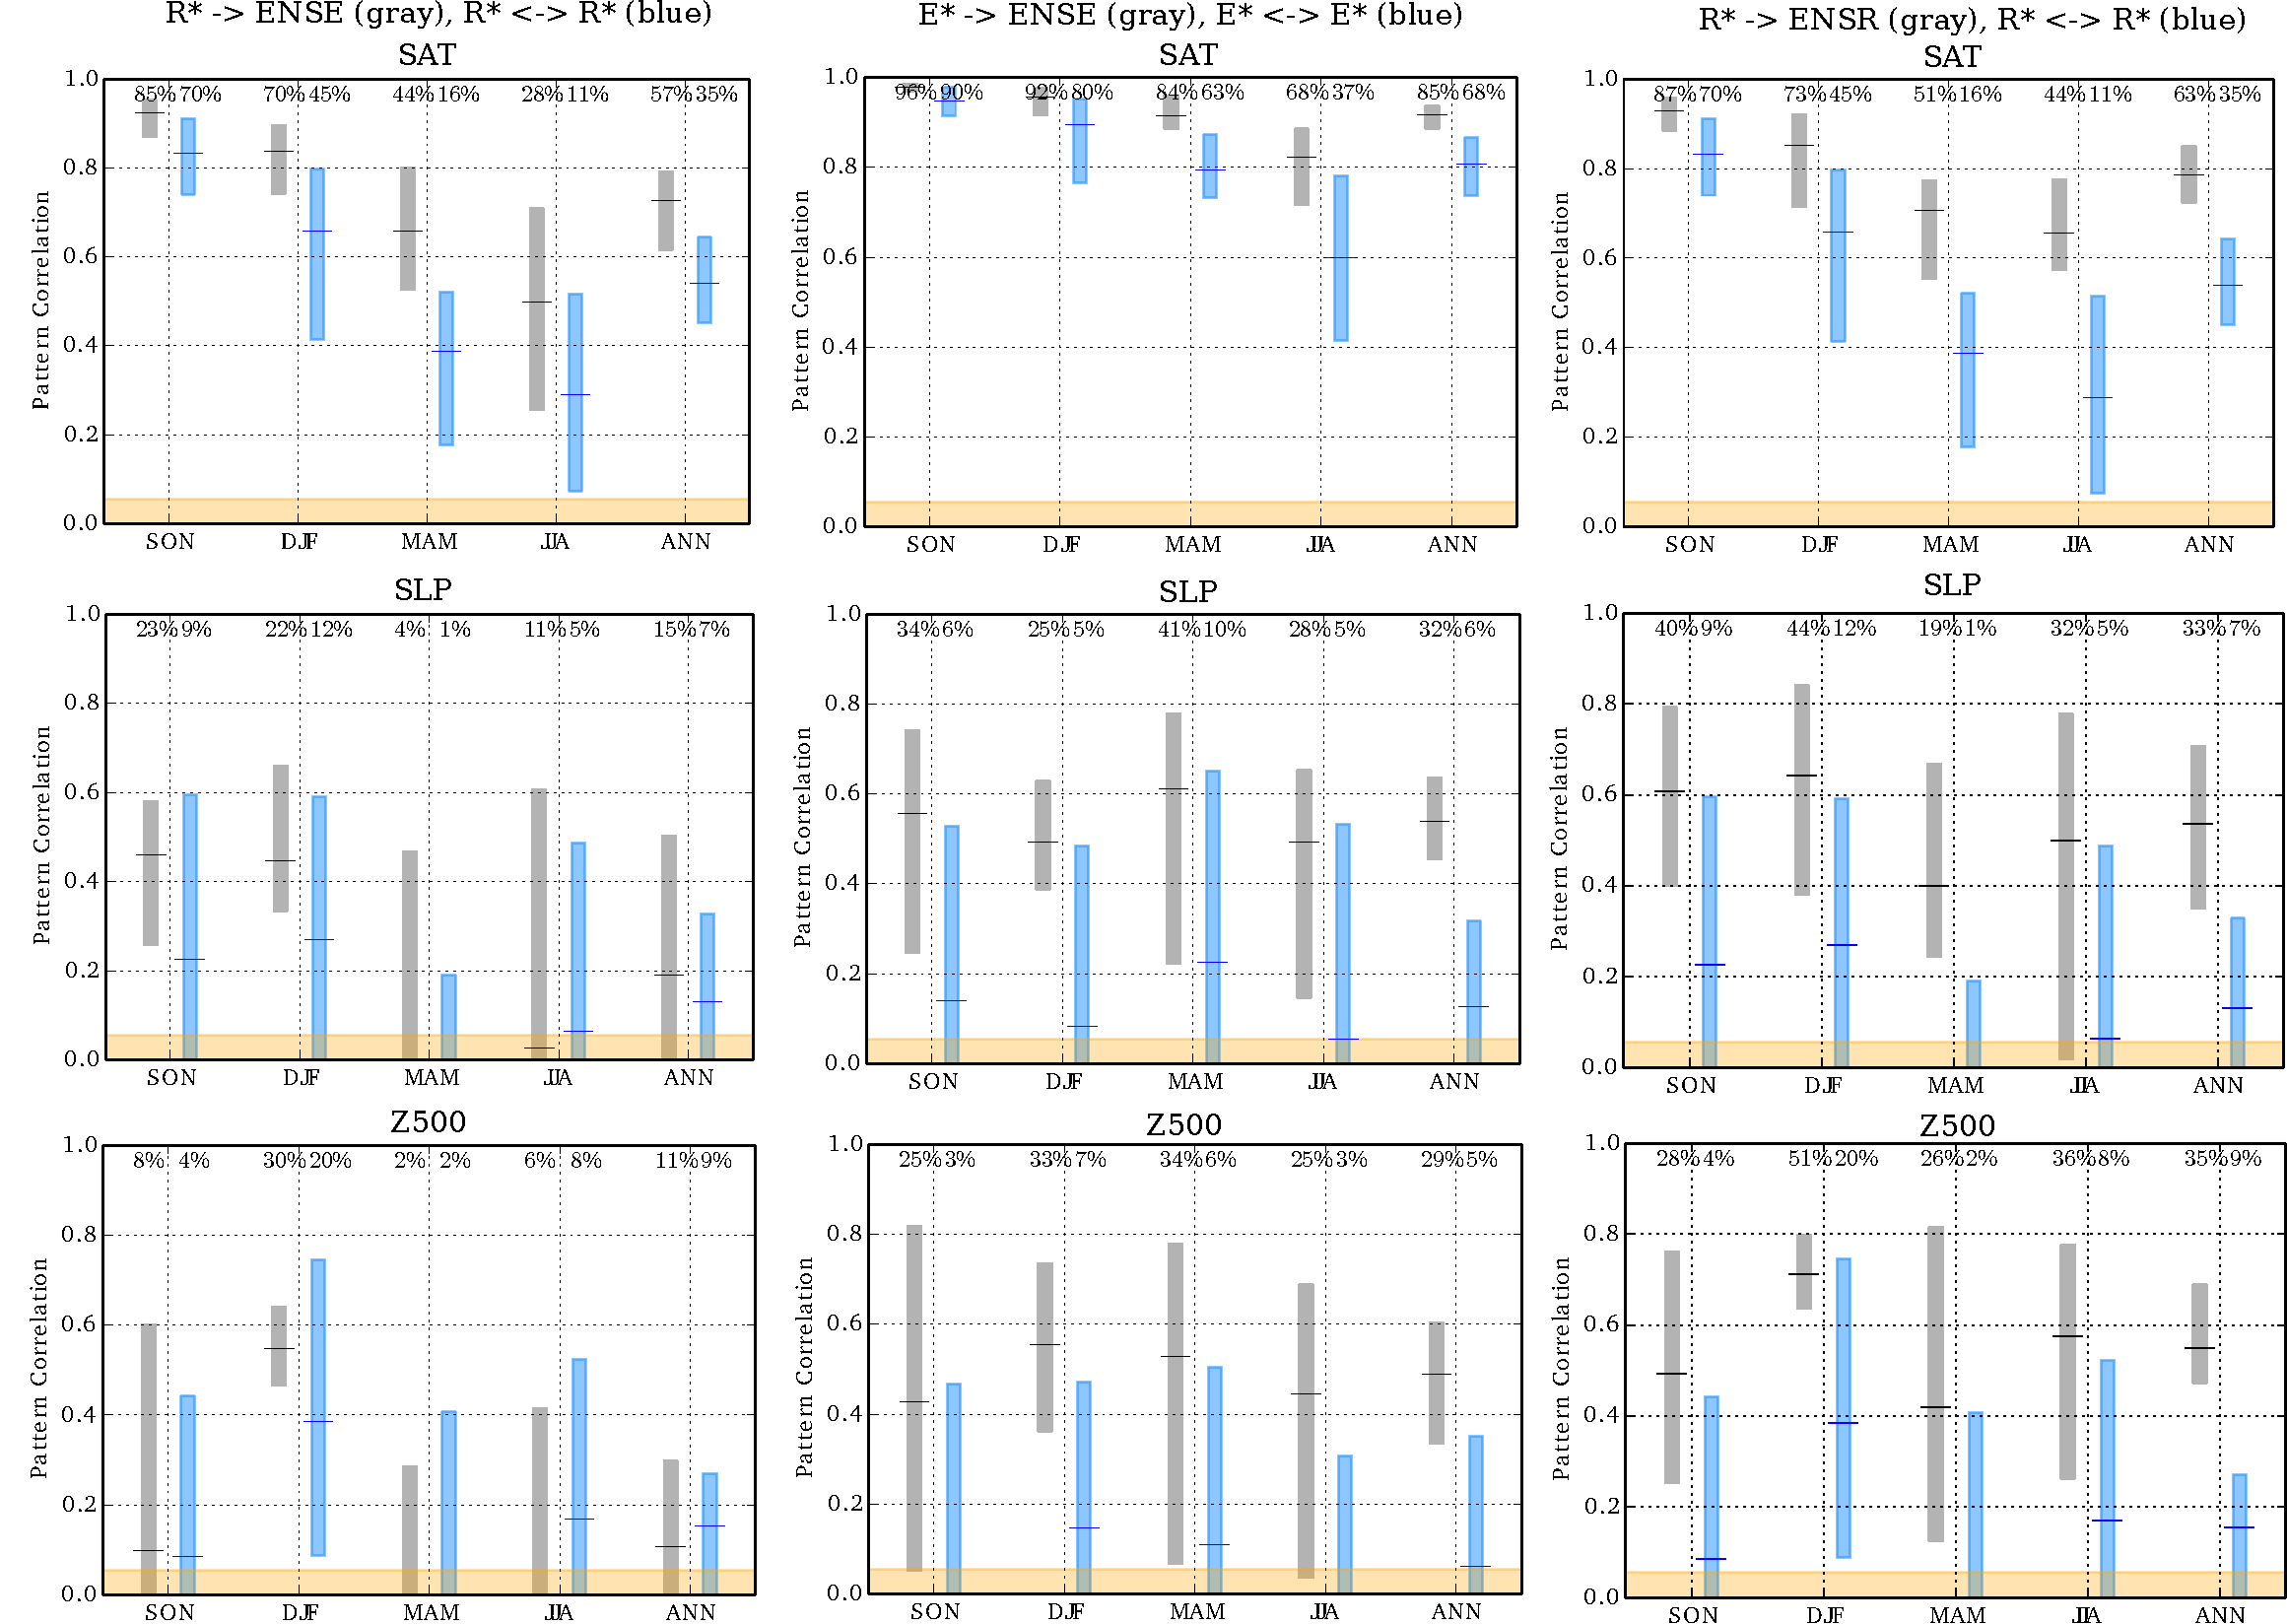
\includegraphics[width=39pc,angle=0]{pattcorrs_rande_ens.pdf}\\
  \caption{Pattern correlations between ensemble members and ensemble means. @@
}\label{fig:pcbars}
\end{figure}


% Create a bibliography directory and place your .bib file there.
\clearpage
\bibliographystyle{./ametsoc}
\bibliography{./references}



\end{document}

